\chapter[Lecture 23]{}\label{lec23}

\section*{Equation of motion}
\begin{figure}[H]
\centering
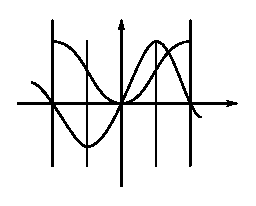
\includegraphics{images/lecture23/fig4.eps}
\end{figure}
Group velocity, $v_{g}=\dfrac{dw}{dk}$\quad $\epsilon=\hbar w$
$$
\therefore\quad v_{g}=\dfrac{1}{\hbar}\dfrac{d\epsilon}{dk}\quad \text{or}\quad \fbox{$\overrightarrow{V}=\dfrac{1}{\hbar}\overrightarrow{\nabla}_{k}\in (k)$}
$$

If a force act on an electon, one can write equation of motion,
$$
F=\hbar \dfrac{dk}{dt}\quad p=\hbar k.
$$
$F$ can be Lorentz force $F=-eE-e\overrightarrow{v}\times \overrightarrow{B}$
$$
\therefore\quad \fbox{$\dfrac{dk}{dt}=-\dfrac{e}{\hbar^{2}}\overrightarrow{\nabla}_{k}\in \times \overrightarrow{B}$}
$$
in a magnetic field. $v=\dfrac{1}{\hbar}\overrightarrow{\nabla}_{k}\in$.

{\em Evidently, election moves on a surface of constant energy if a magnetic field is applied as $\left(\dfrac{dk}{dt}\right)$ is perpendicular to $(\overrightarrow{\nabla}_{k}\epsilon)$}.

\noindent
{\bf Holes:} Vacant state in an otherwise filled band. The properties of holes are as follows.
\begin{itemize}
\item[(i)] In a filled band $\sum k=0$ sum is over all states in the Brillouin zone.

If an electron of momentum $k_{e}$ is ejected, the momentum (total) becomes $-k_{e}$. This is attributed to the hole momentum, $k_{n}:\fbox{$k_{n}=-k_{e}$}$.

An electron of $k_{e}$ wave vector excited at $E$. Total system wave-vector is $-k_{e}$.
\begin{figure}[H]
\centering
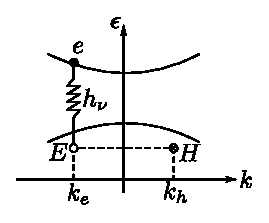
\includegraphics{images/lecture23/fig5.eps}
\end{figure}

But the hole is situated $k_{e}$,

wave vector is graphically situated at $k_{e}$ ($H$ in Fig.) although $k_{n}=-k_{e}$.

\item[(ii)] $\epsilon_{h}(k_{h})=-\epsilon_{e}(k_{e})$

Zero of energy = Fermi energy $\to$ top of valence band. Removal of electron of energy $\epsilon_{e}(k_{e})$ increases the energy of the system by $\epsilon_{e}(k_{e})$ which is the hole energy.

\item[(iii)] Velocity of hole is same as velocity of missing electron.
\begin{gather*}
v_{h}=v_{e}\\
\fbox{$\nabla \epsilon_{h}(k_{n})=\nabla \epsilon_{e}(k_{e})$}\quad\fbox{$v_{h}(k_{h})=v_{e}(k_{e})$}
\end{gather*}

\item[(iv)] $m_{h}=-m_{e}$ effective mass is reversed in sign as hole moves in opposite direction of electron.

\item[(v)] Equation of motion:
$$
\hbar \dfrac{dk_{n}}{dt}=e\left(E+\dfrac{1}{C}v_{h}\times B\right)
$$
Equation of motion of a hole is similar to that of particle of positive charge, `$e$'.
$$
J=(-e)v(G)=(-e)[-v(E)]=ev(E)
$$
Current of a positive charge.
\end{itemize}

\section*{Effective mass}

Mass of an electron in solid is not the same quantity we find in free electrons
$$
\epsilon=\dfrac{\hbar^{2}k^{2}}{2m}
$$
$\to \ \dfrac{1}{m}$ determines the curvature of $\epsilon$ vs. $k$ curve.

One can use similar arguments in solid. Since, the curve is different from free electron behavior, the inertia will be different.
\begin{gather*}
v_{g}=\dfrac{1}{\hbar}\dfrac{d\epsilon}{dk}\quad a, \dfrac{dv_{g}}{dt}=\dfrac{1}{\hbar}\dfrac{d^{2}\epsilon}{dkdt}=\dfrac{1}{\hbar}\dfrac{d^{2}\epsilon}{dk^{2}}\cdot \dfrac{dk}{dt}\\
F=\hbar \dfrac{dk}{dt}\quad \therefore \ \dfrac{dv_{g}}{dt}=\left(\dfrac{1}{\hbar^{2}}\dfrac{d^{2}\epsilon}{dk^{2}}\right)\cdot F=\dfrac{1}{m^{*}}\cdot F.\\
\therefore \ \fbox{$\dfrac{1}{m^{y}}=\dfrac{1}{\hbar^{2}}\dfrac{d^{2}\epsilon}{dk^{2}}$}\quad m^{*} = \text{ effective mass.}
\end{gather*}
If the solid is not isotropic, mass will be a tensor.
$$
\fbox{$\left(\dfrac{1}{m^{*}}\right)_{\mu\nu}=\dfrac{1}{\hbar^{\nu}}\dfrac{d^{2}\epsilon}{dk_{\mu}dk_{\nu}}$}\quad \dfrac{d\nu_{\mu}}{dt}=\left(\dfrac{1}{m^{*}}\right)_{\mu\nu}F_{\nu}
$$
$\mu_{1}\nu$ are cartesian coordinates.

If the band dispersion is flat, the effective mass is very large.

Effective mass often provides a measure of itineracy of the charge carriers. For a local electron, effective mass is infinite.

Effective mass often tells us, how correlated the electrons are $\to$ important measure of electron correlation.

Dirac particles, rest mass is zero, Dispersion is linear.
$$
\epsilon^{2}=p^{2}c^{2}+m^{2}_{0}C^{4}\to m_{0}=0\quad \epsilon\alpha p\text{ or } \epsilon\alpha k\quad \text{ or } p=\hbar k.
$$
\begin{figure}[H]
\centering
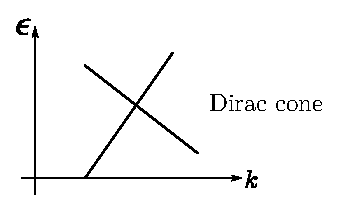
\includegraphics[scale=.85]{images/lecture23/fig6.eps}
\end{figure}
graphene, topological insulators.

\vfill\eject

Density of states : No. of states per unit volume, in the energy range, $(\epsilon)$ and $(\epsilon+d\epsilon)$.

For a solid (cube) of length $L$, total no. allowed states $=\left(\dfrac{L}{2\pi}\right)^{3}\cdot\dfrac{4}{3}\pi k^{3}_{F}\cdot 2$

$k_{F}=$ maximum $k$, upto which levels are filled.
$$
\therefore\quad k_{F}=\left(\dfrac{3\pi^{2}N}{V}\right)^{\frac{1}{3}}
$$
= Fermi wave vector.

Factor 2 is for two spins.

$\therefore$ Fermi energy $\epsilon_{F}=\dfrac{\hbar^{2}k^{2}_{F}}{2m}$.
\begin{align*}
a, \epsilon_{F}=\dfrac{\hbar^{2}}{2m}\left(\dfrac{3\pi^{2}N}{V}\right)^{\frac{2}{3}}\\
v_{F} &= \dfrac{\hbar k_{F}}{m}\\
&= \frac{\hbar}{m}\left(\dfrac{3\pi^{2}N}{V}\right)^{\frac{1}{3}}
\end{align*}
$\therefore$ No. of states filled upto energy $\epsilon$ is
$$
N=\dfrac{V}{3\pi^{2}}\left(\dfrac{2m\epsilon}{\hbar^{2}}\right)^{\frac{3}{2}}\quad \epsilon=\dfrac{\hbar^{2}k^{2}}{2m}.
$$
$$
\therefore\quad \text{Density of states } = \fbox{$D(\epsilon)=\dfrac{dN}{d\epsilon}=\dfrac{V}{2\pi^{2}}\cdot \left(\dfrac{2m}{\hbar^{2}}\right)^{\frac{3}{2}}\cdot \epsilon^{\frac{1}{2}}$}
$$
This is for free electron gas.

In a {\em Semiconductor}, Bands as
\begin{figure}[H]
\centering
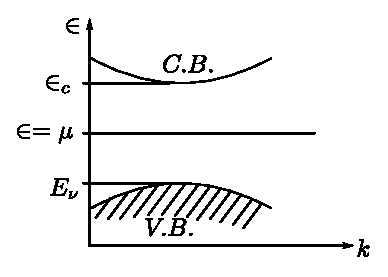
\includegraphics[scale=.85]{images/lecture23/fig7.eps}
\end{figure}

At finite temperature $T$
$$
f_{e}=\dfrac{1}{e^{(\epsilon-\mu)/k_{B^{T}}}+1}
$$

For $k_{B^{T}}\ll \epsilon_{C}-\mu$ which is usually the case,
\begin{align*}
f_{e} &\simeq e^{(\mu-\epsilon)/k_{B^{T}}}\\
\epsilon_{k} &= \epsilon_{C}+\dfrac{\hbar^{2}k^{2}}{2m}
\end{align*}
as the kinetic energy gained by electrons is dependent on how far they are from bottom of conduction band. At band edge, $v_{g}=0\leftarrow \dfrac{d\epsilon}{dk}=0$.
$$
\therefore\quad D_{e}(\epsilon)=\dfrac{1}{2\pi^{2}}\left(\dfrac{2m_{e}}{\hbar^{2}}\right)^{\frac{3}{2}}(\epsilon-\epsilon_{C})^{\frac{1}{2}}\quad V=\text{ unity}
$$
\begin{align*}
\therefore\quad n=\int\limits^{\infty}_{\epsilon_{C}}D_{e}(\epsilon)f_{e}(\epsilon)d\epsilon\\
&= \text{Conduction electrons per unit volume.}\\
&= \frac{1}{2\pi^{2}}\left(\dfrac{2M_{e}}{\hbar^{2}}\right)^{\frac{3}{2}}e^{\frac{\mu}{k_{B^{T}}}}\int\limits^{D}_{\epsilon_{C}}(\epsilon-\epsilon_{C})^{\frac{1}{2}}e^{-\epsilon/k_{B^{T}}}d\epsilon\\
&= 2\left(\dfrac{m_{e}k_{B^{T}}}{2\pi\hbar^{2}}\right)^{\frac{3}{2}}e^{(\mu-\epsilon_{C})/k_{B^{T}}}\tag{A}\label{lec23-eqA}
\end{align*}
For holes,
\begin{align*}
f_{h} &= 1-\dfrac{1}{e^{(\epsilon-\mu)/k_{B^{T}}}+1}=\dfrac{1}{e^{(\mu-\epsilon)/k_{B^{T}}}-1}\\
&\simeq e^{(\epsilon-\mu)/k_{B^{T}}}\quad\text{for}\quad k_{B^{T}}\ll (\mu-\epsilon)
\end{align*}
\begin{align*}
D_{h}(\epsilon) &= \dfrac{1}{2\pi^{2}}\left(\dfrac{2m_{h}}{\hbar^{2}}\right)^{\frac{3}{2}}\\
\therefore \ p &= \int\limits^{\epsilon_{2}}_{-\infty}D_{h}(\epsilon)f_{h}(\epsilon)d\epsilon=2\left(\dfrac{m_{h}k_{B^{T}}}{2\pi\hbar^{2}}\right)^{\frac{3}{2}}e^{(\epsilon_{\nu}-\mu)/k_{B^{T}}}\tag{B}\label{lec23-eq23}
\end{align*}
$$
\therefore\quad \fbox{$n_{p}=4\left(\dfrac{k_{B^{T}}}{\lambda \pi \hbar^{2}}\right)^{3}(m_{e}m_{h})^{\frac{3}{2}}e^{(\epsilon_{\nu}-\epsilon_{C})/k_{B^{T}}}$}
$$
$e-\epsilon_{V}=E_{g} = $ Band gap.

In an intrinsic semiconductor $n=p$.
$$
\therefore\quad \fbox{$n=p=2\left(\dfrac{k_{B^{T}}}{2\pi \hbar^{2}}\right)^{\frac{3}{2}}(m_{e}m_{h})^{\frac{3}{4}}e^{-F_{g}/2k_{B^{T}}}$}
$$
Compare \eqref{lec23-eqA} and \eqref{lec23-eqB}, we get
$$
e^{2\mu/k_{B^{T}}}=\left(\dfrac{m_{h}}{m_{e}}\right)^{\frac{3}{2}}e^{E_{g}/k_{B^{T}}}
$$
$$
a, \ \fbox{$\mu=\frac{1}{2}E_{g}+\frac{3}{4}k_{B^{T}}ln\left(\dfrac{m_{n}}{m_{e}}\right)$}
$$
Fermi level is at the top of the valence band $\to \ E_{\nu}\sim 0$.

For $m_{h}=m_{e}$\quad $\mu=\dfrac{E_{g}}{2}$

$\therefore$ Fermi energy comes at the middle of the gap.

$\nu\to$ velocity = $-eEt$

$F=-eE=\dfrac{d\nu}{dt}m$

Current $J=-ne\nu=+\dfrac{ne^{2}E}{m}$

[no. of electrons passes through unit area per unit time]

$t=\tau$ as electron conduction contribute till it get scattered.

\section*{Mobility}

$\mu=$ Driff velocity of charge carrier per unit electric field.
$$
\mu=|\nu|/E\quad \mu_{e} \text{ \& } \mu_{n}\text{ are both positive.}
$$
Electrical conductivity $\sigma=(ne\mu_{e}+pe\mu_{h})$
\begin{align*}
\nu &= q\tau E/m\\
\therefore\quad \mu_{e} &= \dfrac{e\tau_{e}}{m_{e}}\quad \mu_{h}=\dfrac{e\tau_{h}}{m_{h}}\quad \tau\to \text{ relaxation time.}
\end{align*}

Since temperature dependence of $\tau$ is much weaker than $e^{-Eg/2k_{B^{T}}}$ in semiconductor, the conductivity in such systems are primarily driven be $e^{-Eg/2k_{B^{T}}}$ term.

Holes are less mobile than electrons, due to band degeneracy in the valence band, leading to interband scattering.

Lattice distortion induced energy band modification Jahn-Teller distortion etc.
\begin{figure}[H]
\centering
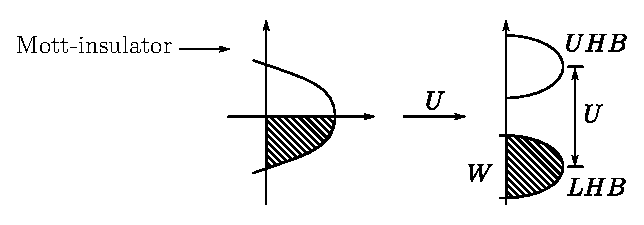
\includegraphics[scale=.85]{images/lecture23/fig8.eps}
\end{figure}
$\dfrac{U}{W}>1$ insulator

\medskip

$\dfrac{U}{W}<1$ metal

\medskip

Band gap $\sim U-W$



 
